\chapter*{Introduction \& problem definition}
This is the report of Paolo Ginefra's solution to the "Image Analysis and Computer Vision" homework 2024/25.
All the referenced code is available in the GitHub Repository.

\section{Problem definition}
In this section, the problem at hand will be described in detail referencing the "Homework Assignment 2024-25" document.
\subsection{Scene description}
 A piece of furniture is a rectangular parallelepiped, whose width (along the X-axis) is $l = 1$. 
The other dimensions, namely the depth $m$ along the $Y$ axis and the height $h$ along the $Z$-axis are 
unknown. In addition, a horizontal circumference (i.e., parallel to the X-Y plane) is visible. 
Furthermore, an unknown horizontal planar curve is also visible, placed at midheight $h$/2. 

\begin{figure}[!ht]
\centering
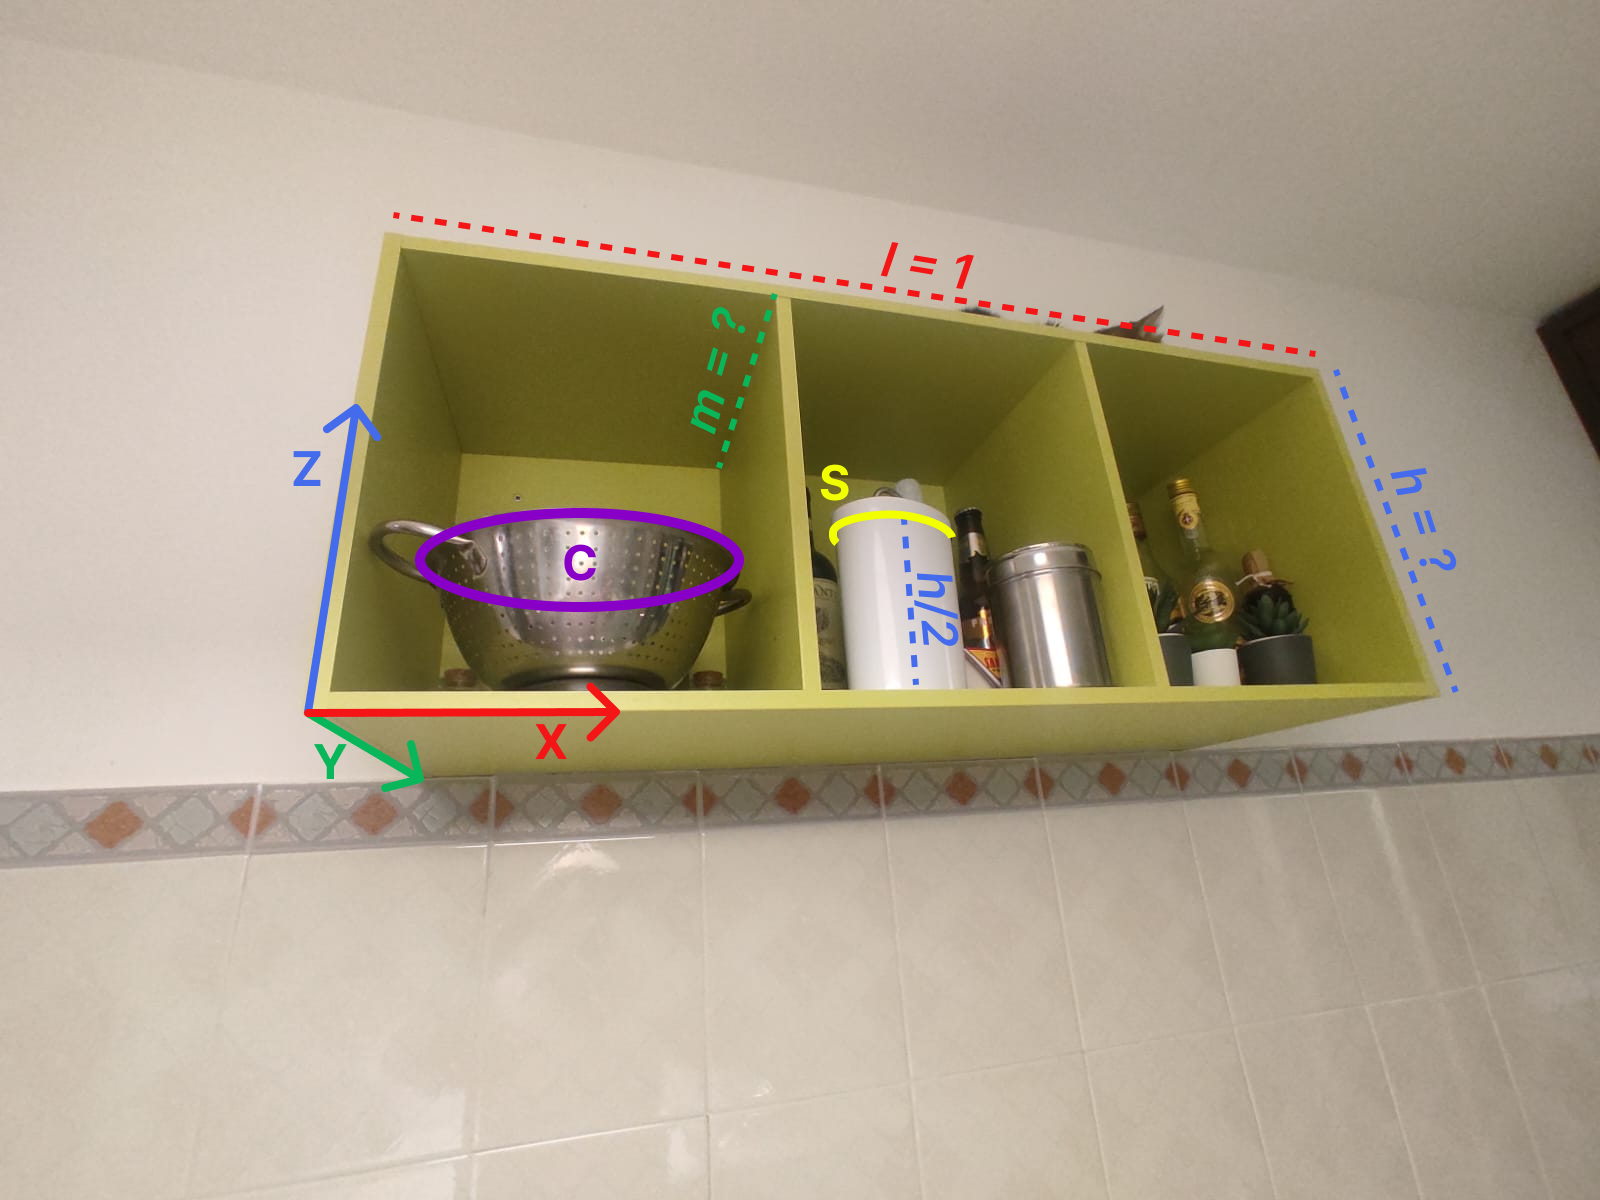
\includegraphics[height=9.5cm, width=\textwidth, keepaspectratio]{Report/Images/Introduction/Scene Description.png}
\caption{\label{fig:SceneDescription}The Scene Description}
\end{figure}

\subsection{Image Description}
A single image is taken of the above rectangular parallelepiped by an uncalibrated, zero
skew, camera. (Its calibration matrix $K$ depends on four unknown parameters, namely $f_x$, $f_y$ and 
the two pixel coordinates $U_O$, $V_O$ of the principal point). A set of lines parallel to X-axis are visible, and their images $l_1$, $l_2$ and $l_3$ are extracted; a set of lines parallel to the $Y$-axis are visible and their images  $m_1$, $m_2$, $m_3$, $m_4$, $m_5$ and $m_6$ are extracted; a set of vertical lines (i.e., parallel to the $Z$
axis) are also visible and their images $h_1$, $h_2$, $h_3$ and $h_4$ are extracted.  In addition, both the image $C$ of the circumference and the image $S$ of the unknown horizontal curve are also extracted.  

